\documentclass[notitlepage]{revtex4-2}
\usepackage[utf8]{inputenc}
\usepackage{geometry}
\usepackage{xcolor}
\geometry{a4paper, margin=1in}
\usepackage{graphicx}
\usepackage{amsmath}
\usepackage[margin=5pt]{subfig}
\definecolor{darkgreen}{rgb}{0.00,0.50,0.25}
\definecolor{darkblue}{rgb}{0.00,0.00,0.67}
\usepackage[breaklinks,pdftitle={Analysis of VE-Model and Buyback and Burn Model}, pdfauthor={Oleg Zakharchenko},colorlinks,urlcolor=blue,citecolor=darkgreen,linkcolor=darkblue]{hyperref}
\graphicspath{{pdf/}}

\setkeys{Gin}{scale=0.5}

\begin{document}

% Title Page
    \begin{titlepage}
        \centering
        
\includegraphics[width=0.3\textwidth]{images/curve-dao-token-crv-logo}\\[1cm]
        \rule{\textwidth}{0.5mm}\\[0.5cm]
        {\Large A Comparative Analysis of VE-Model and Buyback and Burn Model for DeFi Tokenomics: Curve.fi example}\\[0.5cm]
        \rule{\textwidth}{0.5mm}\\[1.5cm]

        \textbf{Author:}\\
        Oleg Zakharchenko \\[1cm]
        Curve.fi \\[1cm]

        \vfill
        \textbf{Date of Publication:}\\
        April 2025\\[1cm]

        \href{https://curve.fi}{curve.fi}\\
    \end{titlepage}


% Sections

\begin{abstract}
    Decentralized Finance (DeFi) projects have evolved significantly in recent years, leveraging innovative tokenomics
    models to enhance governance and value capture for participants.
    Among the most prominent models are the Voting Escrow (VE) model and the Buyback model, each offering distinct
    approaches to incentivizing token holders and managing project sustainability.
    The VE model emphasizes long-term commitment by locking tokens to gain governance rights and increased rewards,
    fostering alignment between token holders and the project’s long-term success.
    On the other hand, the Buyback and Burn model seeks to directly boost token value by repurchasing tokens from the market,
    reducing supply and thereby increasing scarcity.
    This paper aims to provide a comprehensive comparison of these two models based on tokenomics and data for Curve.fi
    for the past 4 years.
    Results show that VE-model provides more long-term value impact for token scarcity alongside it's value to provide
    governance rights and increased rewards.
\end{abstract}

\section{Introduction}
The exponential growth of Decentralized Finance (DeFi) has introduced diverse tokenomics strategies that seek to align
user incentives, foster active governance, and promote long-term project sustainability. Among the prominent approaches
are the Voting Escrow (VE) model and the Buyback model, each offering distinctive methods for incentivizing token
holders and contributing to project longevity.
The VE model emphasizes governance through commitment, where token holders lock their tokens over extended periods in
exchange for voting power and increased rewards. This model, widely adopted by several DeFi projects,
promotes a strong alignment between token holders and the long-term goals of the project. In contrast, the Buyback
model focuses on direct token value accrual by repurchasing tokens from the market to decrease supply and increase
scarcity, thereby potentially boosting token prices.
This article aims to analyze and compare these two models, assessing their implications on governance, value
distribution, and overall project success. By evaluating the strengths and weaknesses of each approach, this analysis
seeks to find which model may be best suited best for Curve based on real data obtained since project launch in 2020.

\section{Bribes as Incentives for veCRV Holders}

In the context of decentralized governance, bribes have emerged as a controversial yet effective mechanism to influence
voting behavior, especially among veCRV holders. The veCRV model, integral to the Curve Finance ecosystem, grants
voting power based on the duration of token lock-up, with longer lock-up periods translating to greater voting
influence. This governance structure encourages a vested interest in the platform’s long-term success, aligning token
holders' incentives with sustainable growth.

Bribes, however, add an additional layer of incentives by directly rewarding veCRV holders to vote in a particular way.
Through bribes, external projects or protocols can incentivize veCRV holders to support specific proposals,
liquidity pools, or strategic initiatives that align with the interests of the bribe-givers. These bribes are typically
offered as additional token rewards or financial incentives that holders receive upon voting as requested.

To facilitate and streamline the bribing process, several platforms, known as vote markets, exist, allowing
veCRV holders to efficiently exchange their voting power for incentives. Below, we explore five prominent vote markets
for veCRV holders - this is \textbf{bribe.crv.finance}, \textbf{VoteMarket}, \textbf{Votium}, \textbf{Quest} and
\textbf{yBribe}.

\begin{figure}[ht]
    \centering
    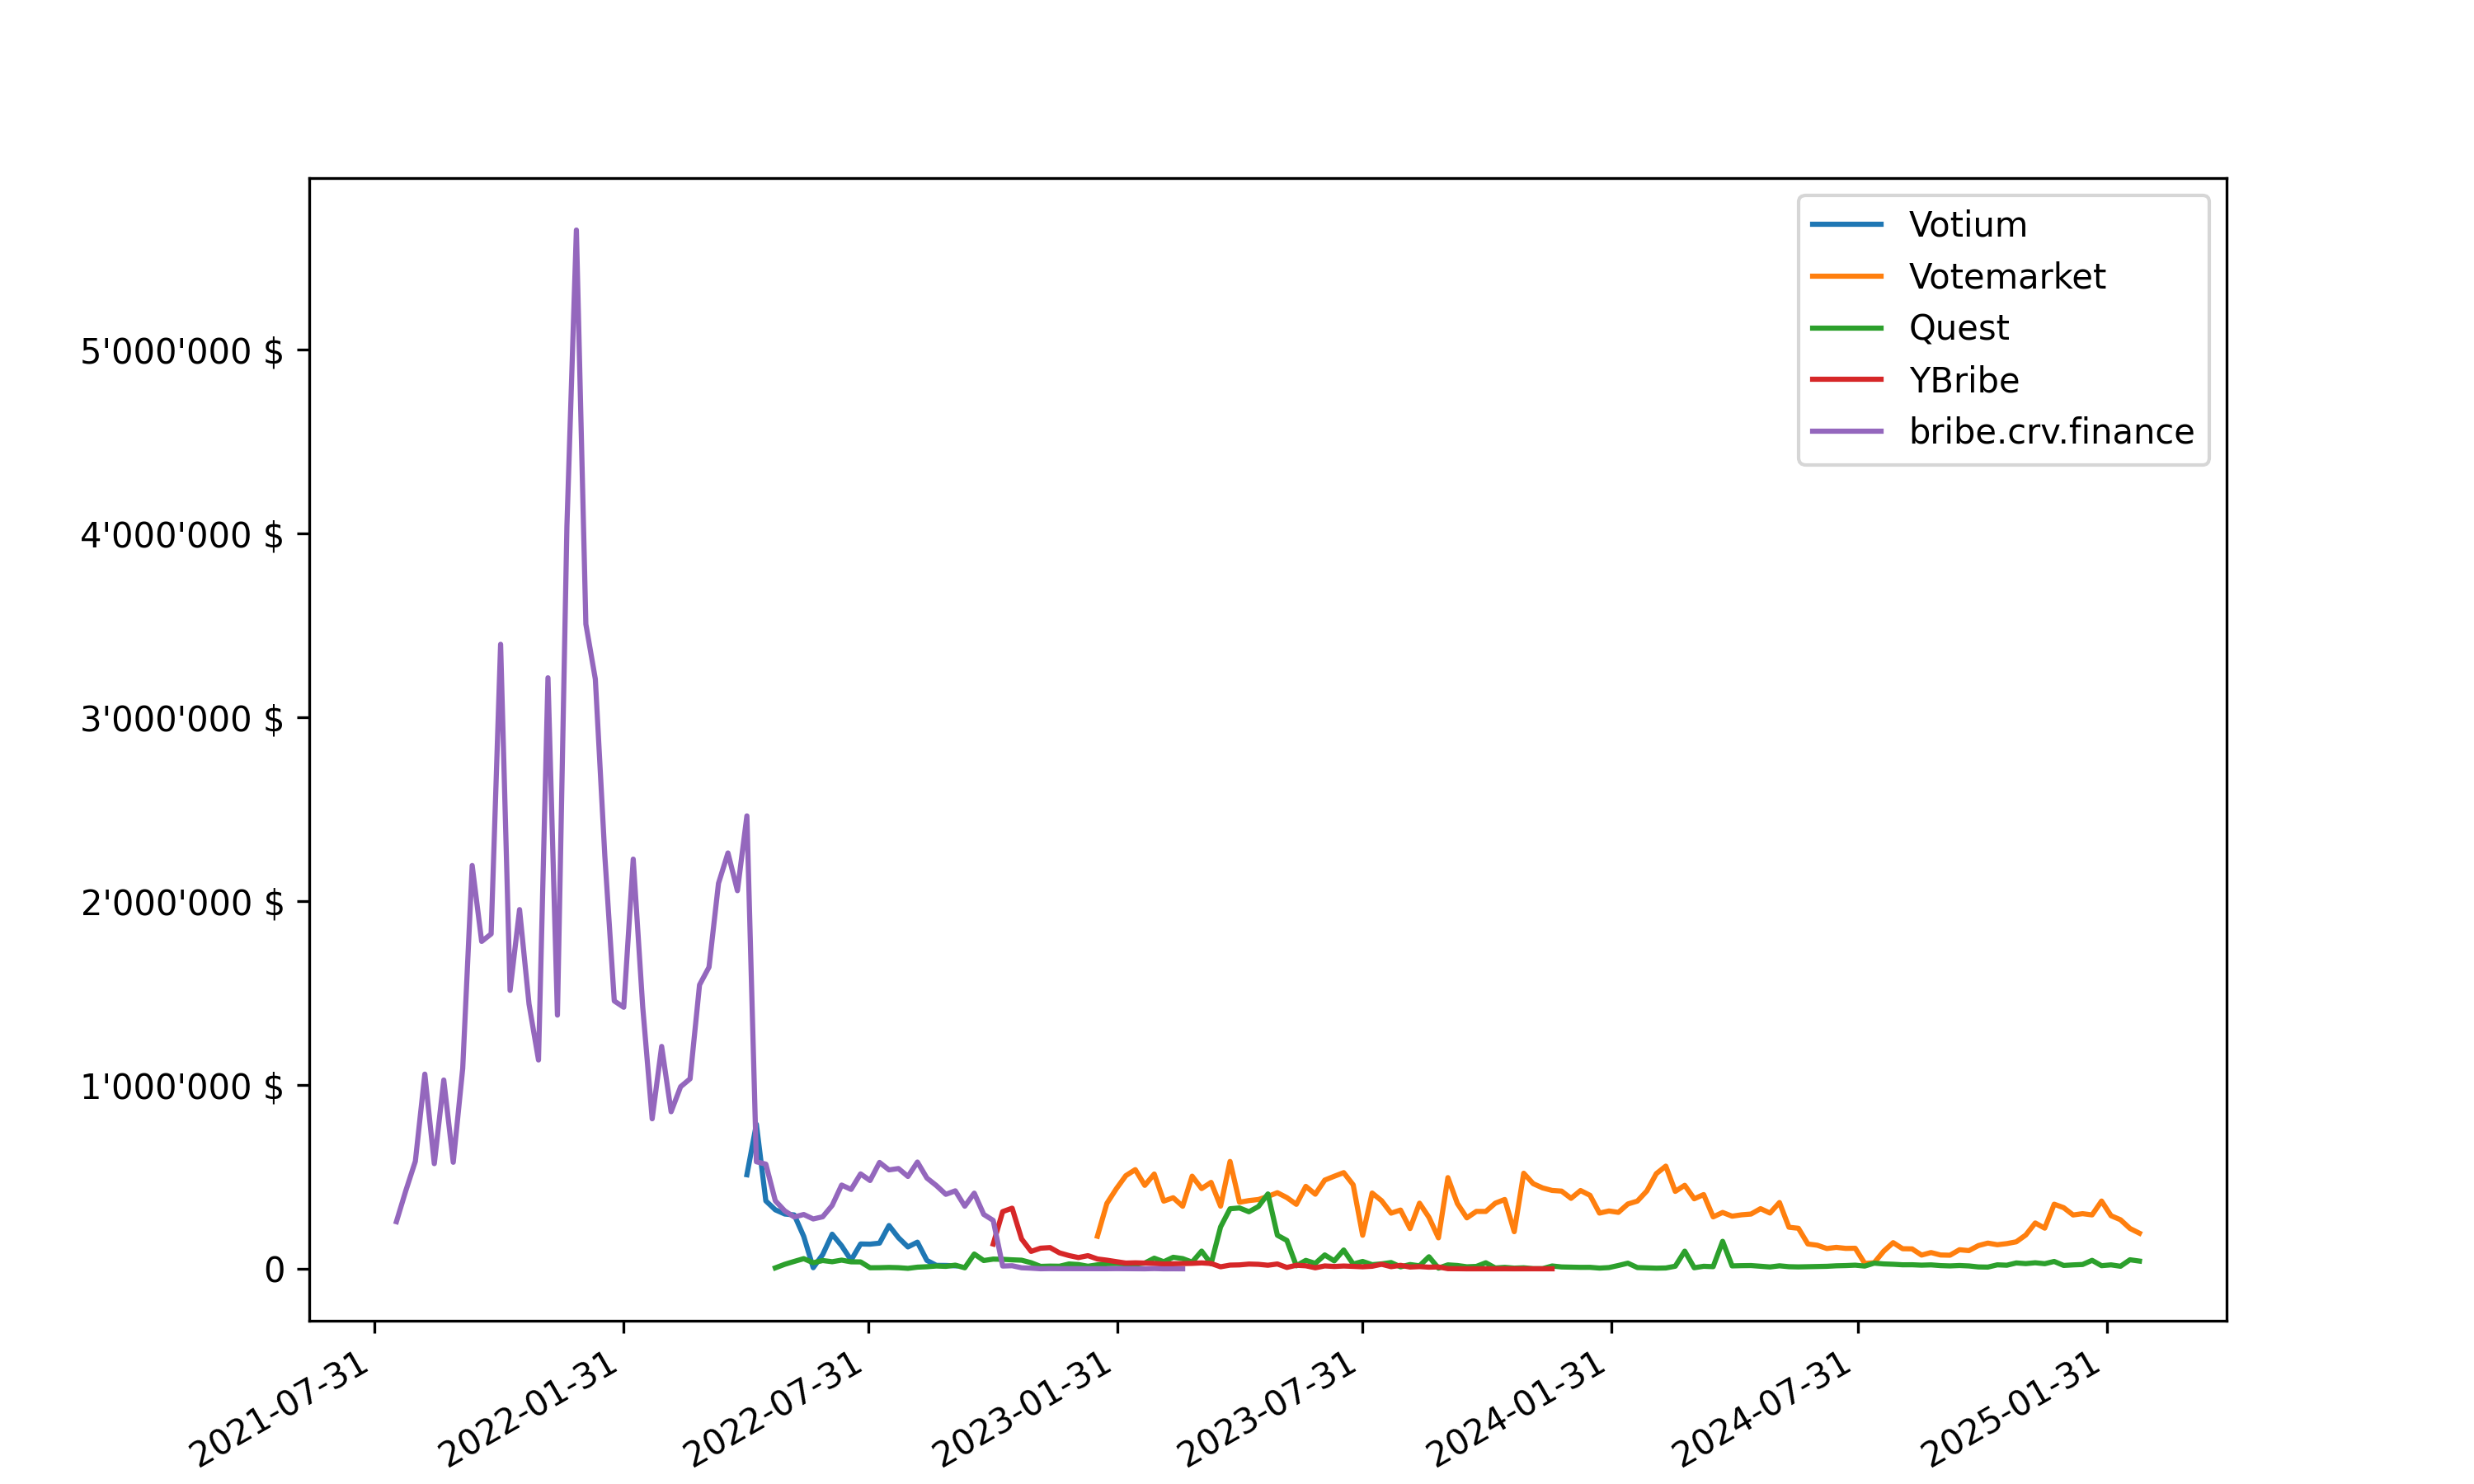
\includegraphics[width=\linewidth]{images/CRV_bribes_comparison}
    \caption{Distribution of Curve bribes from different sources. Source: \href{https://crvhub.com}{CRVHub}}
    \label{fig:bribes_distribution}
\end{figure}

Developed by the Curve Finance team as first version, bribe.crv.finance was initially integrated directly into
the Curve platform, providing projects and protocols with a streamlined mechanism to offer bribes for veCRV votes.
As illustrated in Figure 1, this platform served as the primary revenue source for veCRV holders during its period
of active use. Subsequently, Curve Finance transitioned to utilizing external voting platforms, effectively outsourcing
the bribing mechanism and ceasing the use of its proprietary platform.

Among the external options, VoteMarket emerged as the dominant platform in terms of transaction volume. Operating
independently, VoteMarket facilitates a broad range of DeFi projects in posting bribes for veCRV holders. As shown in
Figure \ref{fig:bribes_distribution}, VoteMarket’s transaction volumes closely mirror those seen in the final stages of
bribe.curve.fi’s operation, indicating a shift of activity to this platform. Overall, the data reveal that bribing
volumes remained stable from the second half of 2022 through 2023, with a decline observed in 2024.

\section{Curve.fi Revenue from Pool Activity and crvUSD Markets}

\begin{figure}[ht]
    \centering
    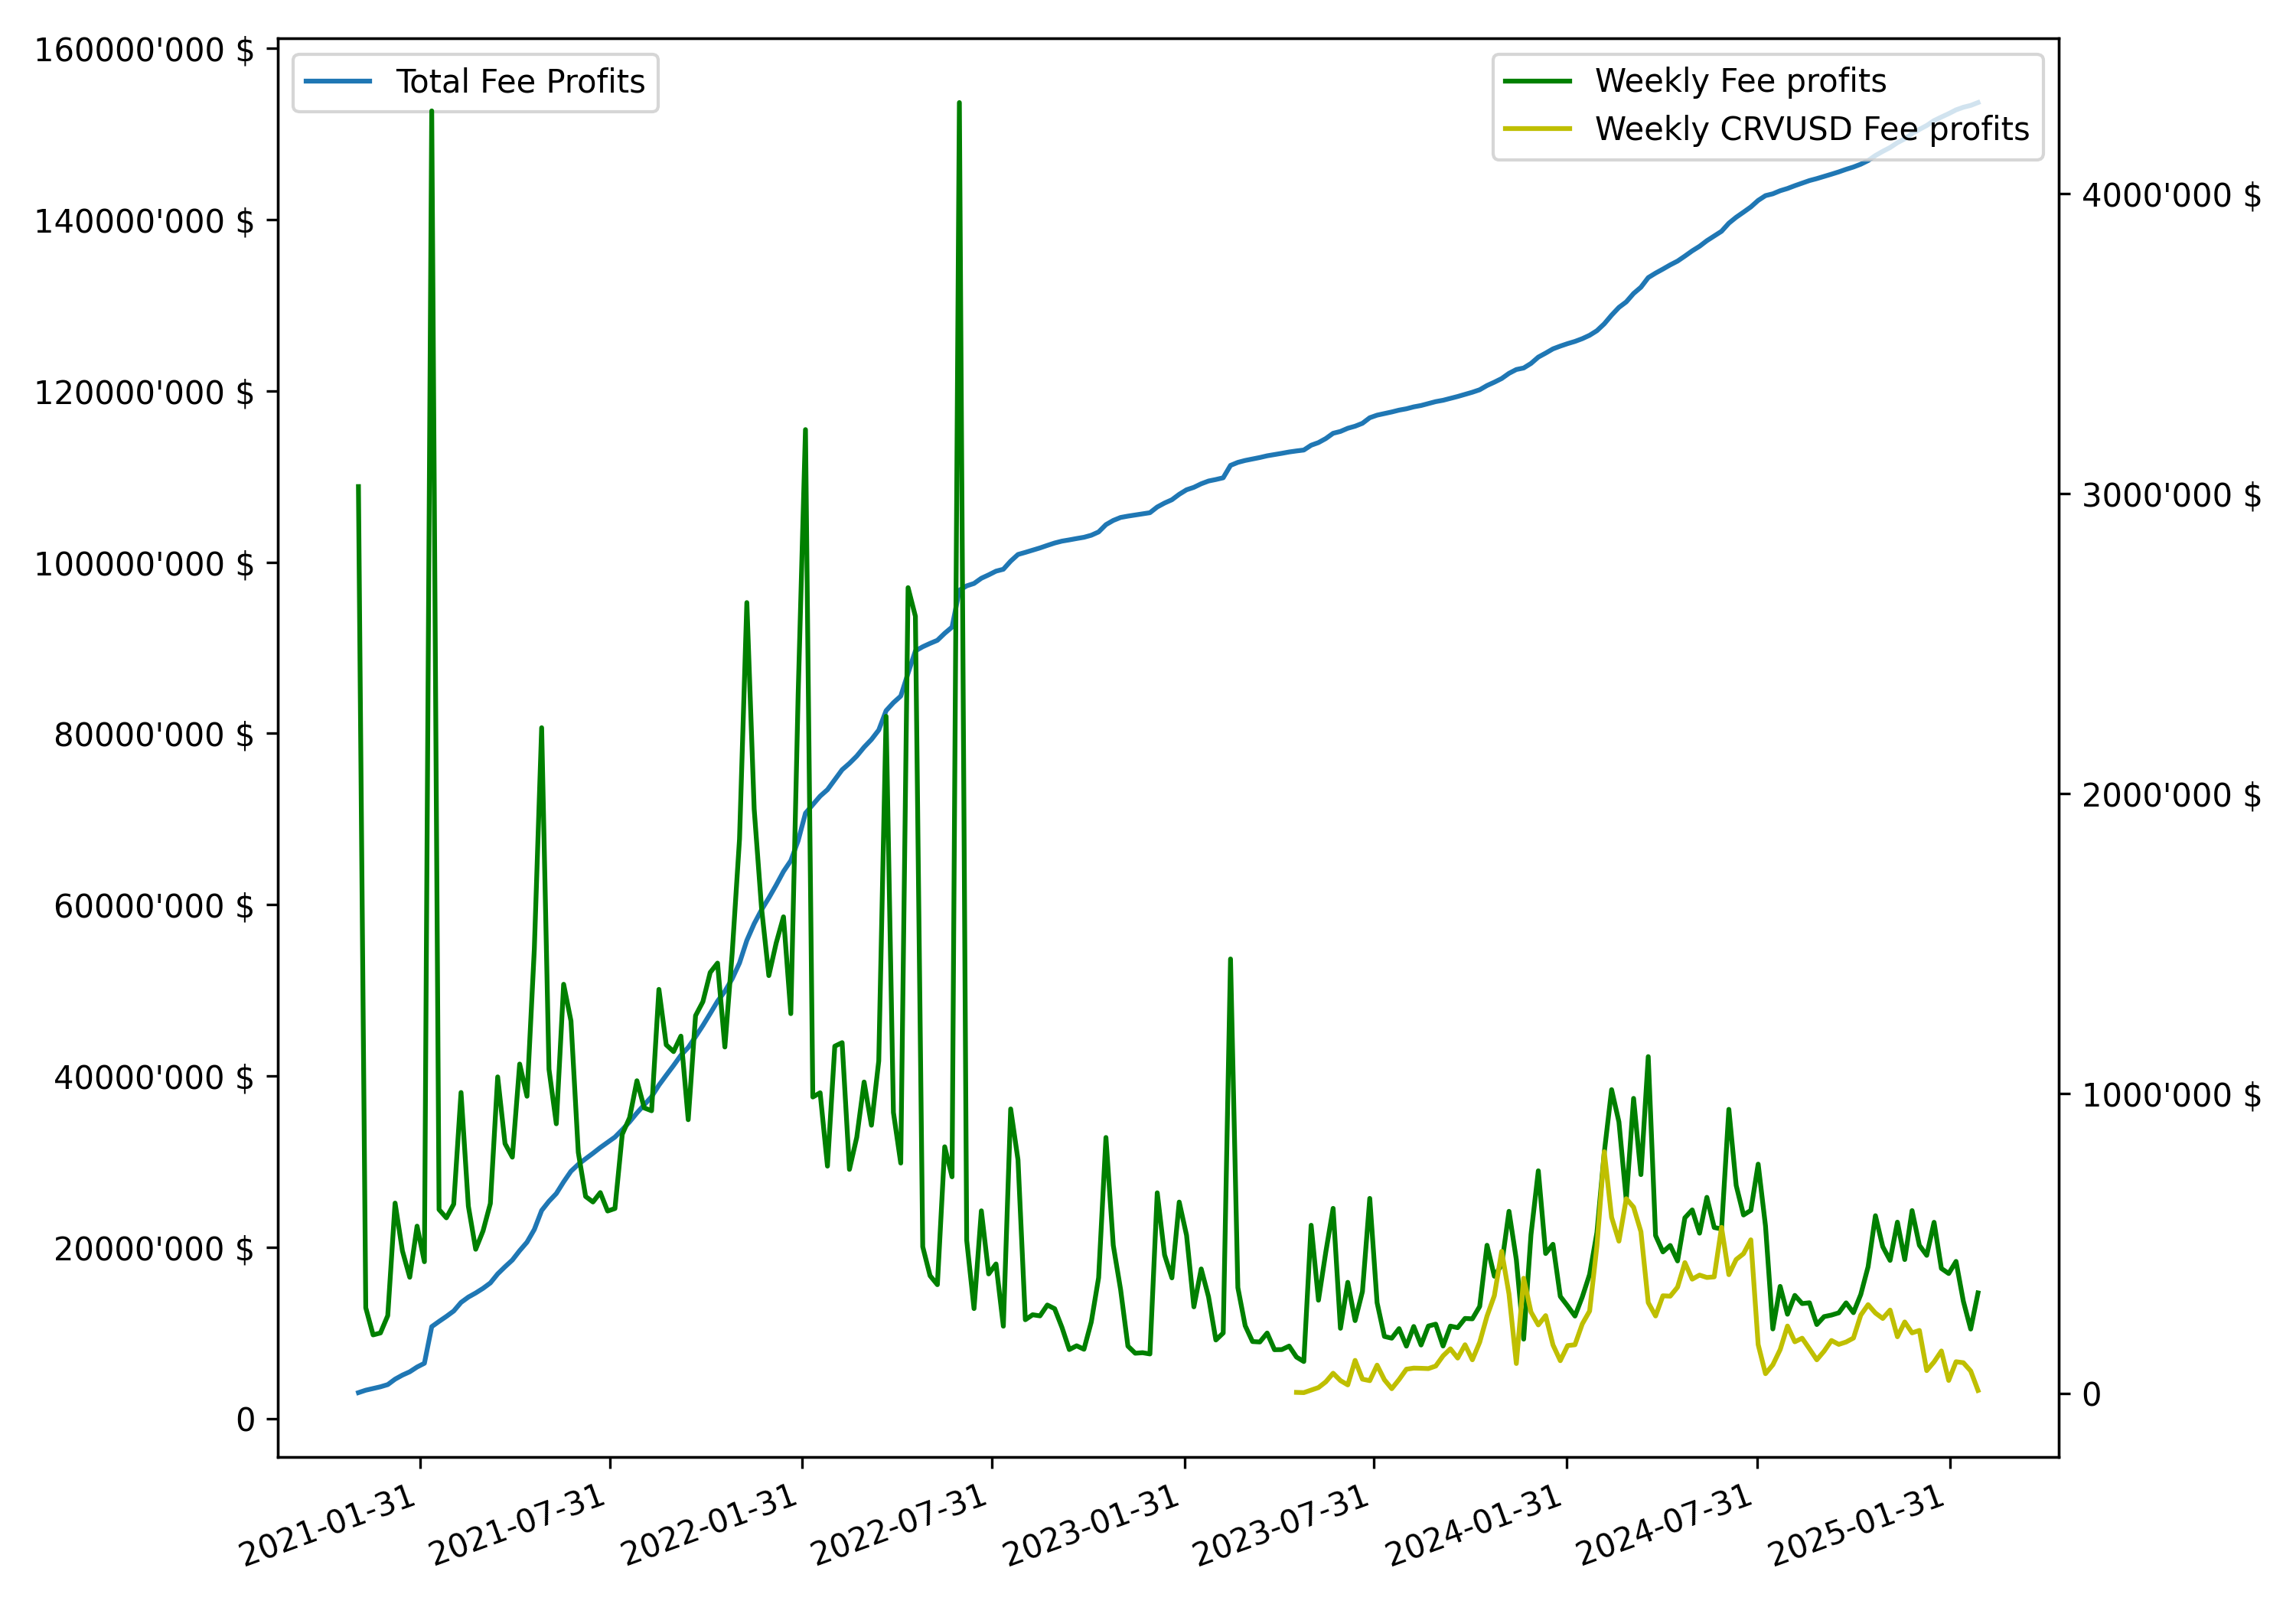
\includegraphics[width=\linewidth]{images/CRV_fee}
    \caption{Distribution of fee amounts from protocol.}
    \label{fig:fee_distribution}
\end{figure}

Starting from 2023, fees generated from pool activity became the primary source of revenue for the Curve.fi platform,
surpassing bribes in terms of volume. The bulk of Curve’s fees originates from its core functionality: stablecoin and
asset pools designed for efficient, low-slippage trades. These pools attract high trading volumes by offering
competitive exchange rates for stablecoins and other assets, which in turn generates consistent fee income for the
platform. As trading activity increased in 2023, particularly with the introduction of additional stablecoin pools,
revenue from pool fees rose sharply (Figure \ref{fig:fee_distribution}).

In addition to traditional pool fees, Curve’s introduction of the crvUSD stablecoin markets has added a new revenue
stream. crvUSD is designed as a decentralized, over-collateralized stablecoin, and its issuance and trading activities
bring substantial fee income to Curve. By supporting crvUSD across multiple pools, Curve has enhanced both trading
volume and user engagement on the platform. The crvUSD markets allow Curve to capture fees not only from asset swaps
but also from lending and borrowing activities associated with the stablecoin, adding a layer of revenue that was
previously absent from the platform’s fee structure.

\begin{figure}[ht]
    \centering
    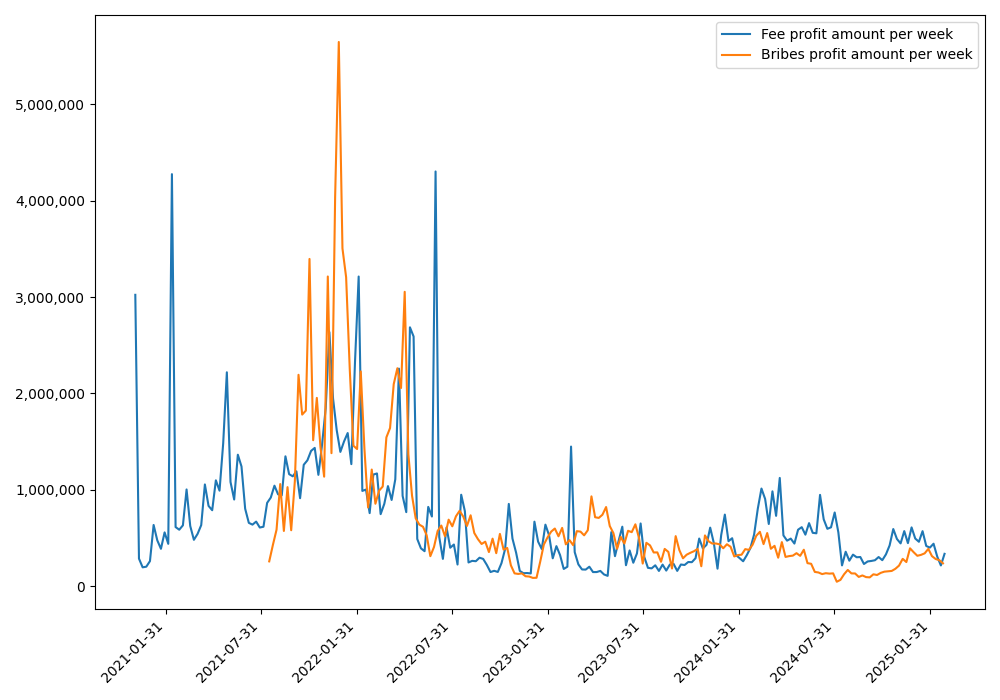
\includegraphics[width=\linewidth]{images/CRV_profits}
    \caption{Overall profits from bribes and fees. Bribes volume source: \href{https://crvhub.com}{CRVHub}}
    \label{fig:profits}
\end{figure}

Compared to the earlier dominance of bribes as a revenue source, fees from pool activity and crvUSD markets offer a
more sustainable and scalable model for Curve’s long-term growth. While bribes provided significant revenue during
their peak, they are inherently tied to the interests of external protocols seeking governance influence. In contrast,
transaction fees from pools and crvUSD markets are aligned with organic trading activity and user participation within
the Curve ecosystem itself. As shown in Figure \ref{fig:profits}, revenue from fees consistently outpaced bribe income
from 2023 onwards, illustrating a marked shift in Curve’s revenue composition.

In summary, the increased reliance on fees from pool activity and crvUSD markets has established a more balanced and
enduring revenue model for Curve, with long-term benefits for both the platform and its community of veCRV holders.

\section{Comparison of Burn Model vs. veCRV Model: Token Scarcity and Value Accrual}

The tokenomics of DeFi protocols are crucial in determining how value is distributed among participants and how
governance power is allocated. Two prominent models that have gained traction in DeFi are the \textbf{burn model} and
the \textbf{veCRV model}. Both approaches aim to create token scarcity and drive value to token holders, yet they
operate through fundamentally different mechanisms.

\begin{figure}[ht]
    \centering
    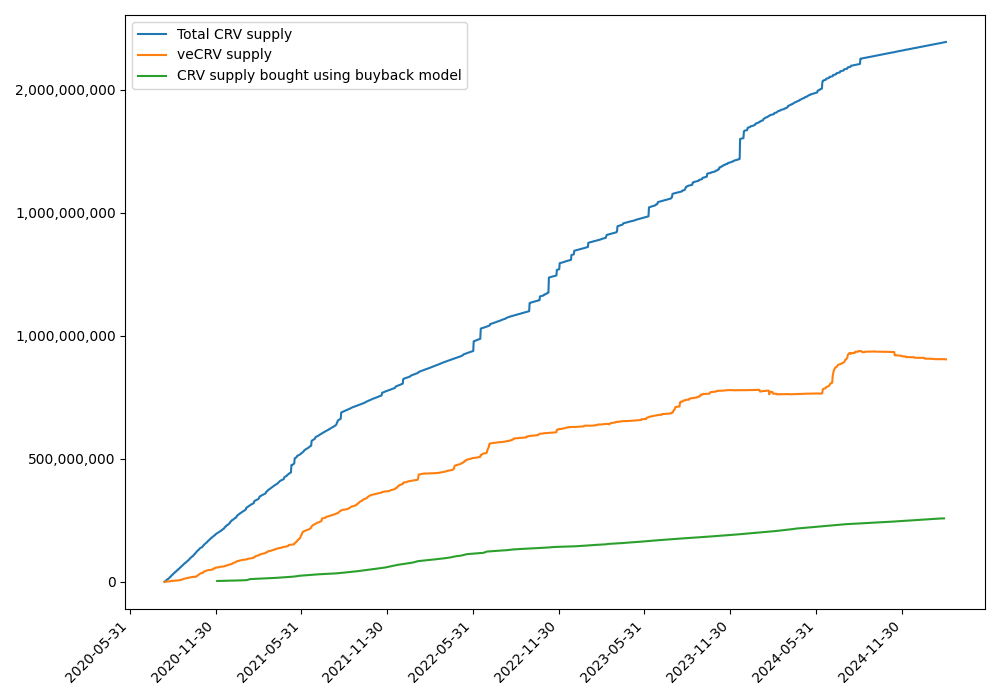
\includegraphics[width=\linewidth]{images/CRV_burn_model}
    \caption{CRV(1), veCRV(2) and potentially bought from fees and bribes CRV amounts.}
    \label{fig:vecrv}
\end{figure}

The burn model reduces token supply by permanently removing tokens through buybacks and burns, often funded by protocol
revenue. By decreasing the circulating supply, the burn model aims to increase token scarcity and, theoretically,
drive up the value of the remaining tokens. Many DeFi protocols adopt this model to offer a straightforward value
accrual mechanism to token holders, as each burn directly reduces the available token supply.

In contrast to the burn model, the veCRV model is based on token locking rather than permanent removal. Within this
model, users lock CRV tokens in the Curve protocol in exchange for veCRV, which confer voting rights and increased
reward payouts. The locked tokens remain in the protocol, effectively reducing circulating supply while providing
governance incentives for long-term holders. Unlike the burn model, which creates scarcity through destruction,
the veCRV model incentivizes users to hold tokens over extended periods, aligning holder interests with the protocol’s
growth. The data reveals that this model locks approximately three times more tokens than would be removed through
a burn mechanism (Figure \ref{fig:vecrv}), illustrating its superior impact on token scarcity. Despite the
non-permanent nature of veCRV locks, which range from 0 to 4 years without completely removing tokens from circulation,
the supply of veCRV has shown steady growth. This trend indicates that market participants, including aggregators like
Convex Finance, recognize and value the scarcity created by veCRV locking.

Ultimately, while the burn model offers an accessible approach to token scarcity, the veCRV model, especially when
coupled with aggregators, provides a more comprehensive framework for achieving scarcity and enhancing governance.
With three times the token volume locked in veCRV compared to potential burns, Curve’s veCRV model demonstrates a
robust mechanism for aligning user incentives with protocol growth, indicating that token locking may hold greater
advantages for sustainable DeFi ecosystem development. This includes: users gaining voting power and a say in protocol
decisions, which enhances decentralized governance; users receiving additional incentives such as boosted yields and a
share in protocol fees (which was discussed above) and users directry receiving their rewards equal to their commitment
to the protocol’s success and longevity. This model promotes a more engaged and long-term oriented community,
addressing common issues in DeFi related to short-term speculation and governance exploitation.

\section{Special thanks.}

Special thanks to Michael Egorov from Curve and team from Aragon for reviewing the article and
\href{https://crvhub.com}{CRVHub} team for providing Bribes data for veCRV.

\end{document}
